\documentclass{standalone}
\usepackage{tikz}
\usetikzlibrary{patterns, positioning}
\usepackage[sfdefault]{ClearSans} %% option 'sfdefault' activates Clear Sans as the default text font
\usepackage[T1]{fontenc}

\begin{document}
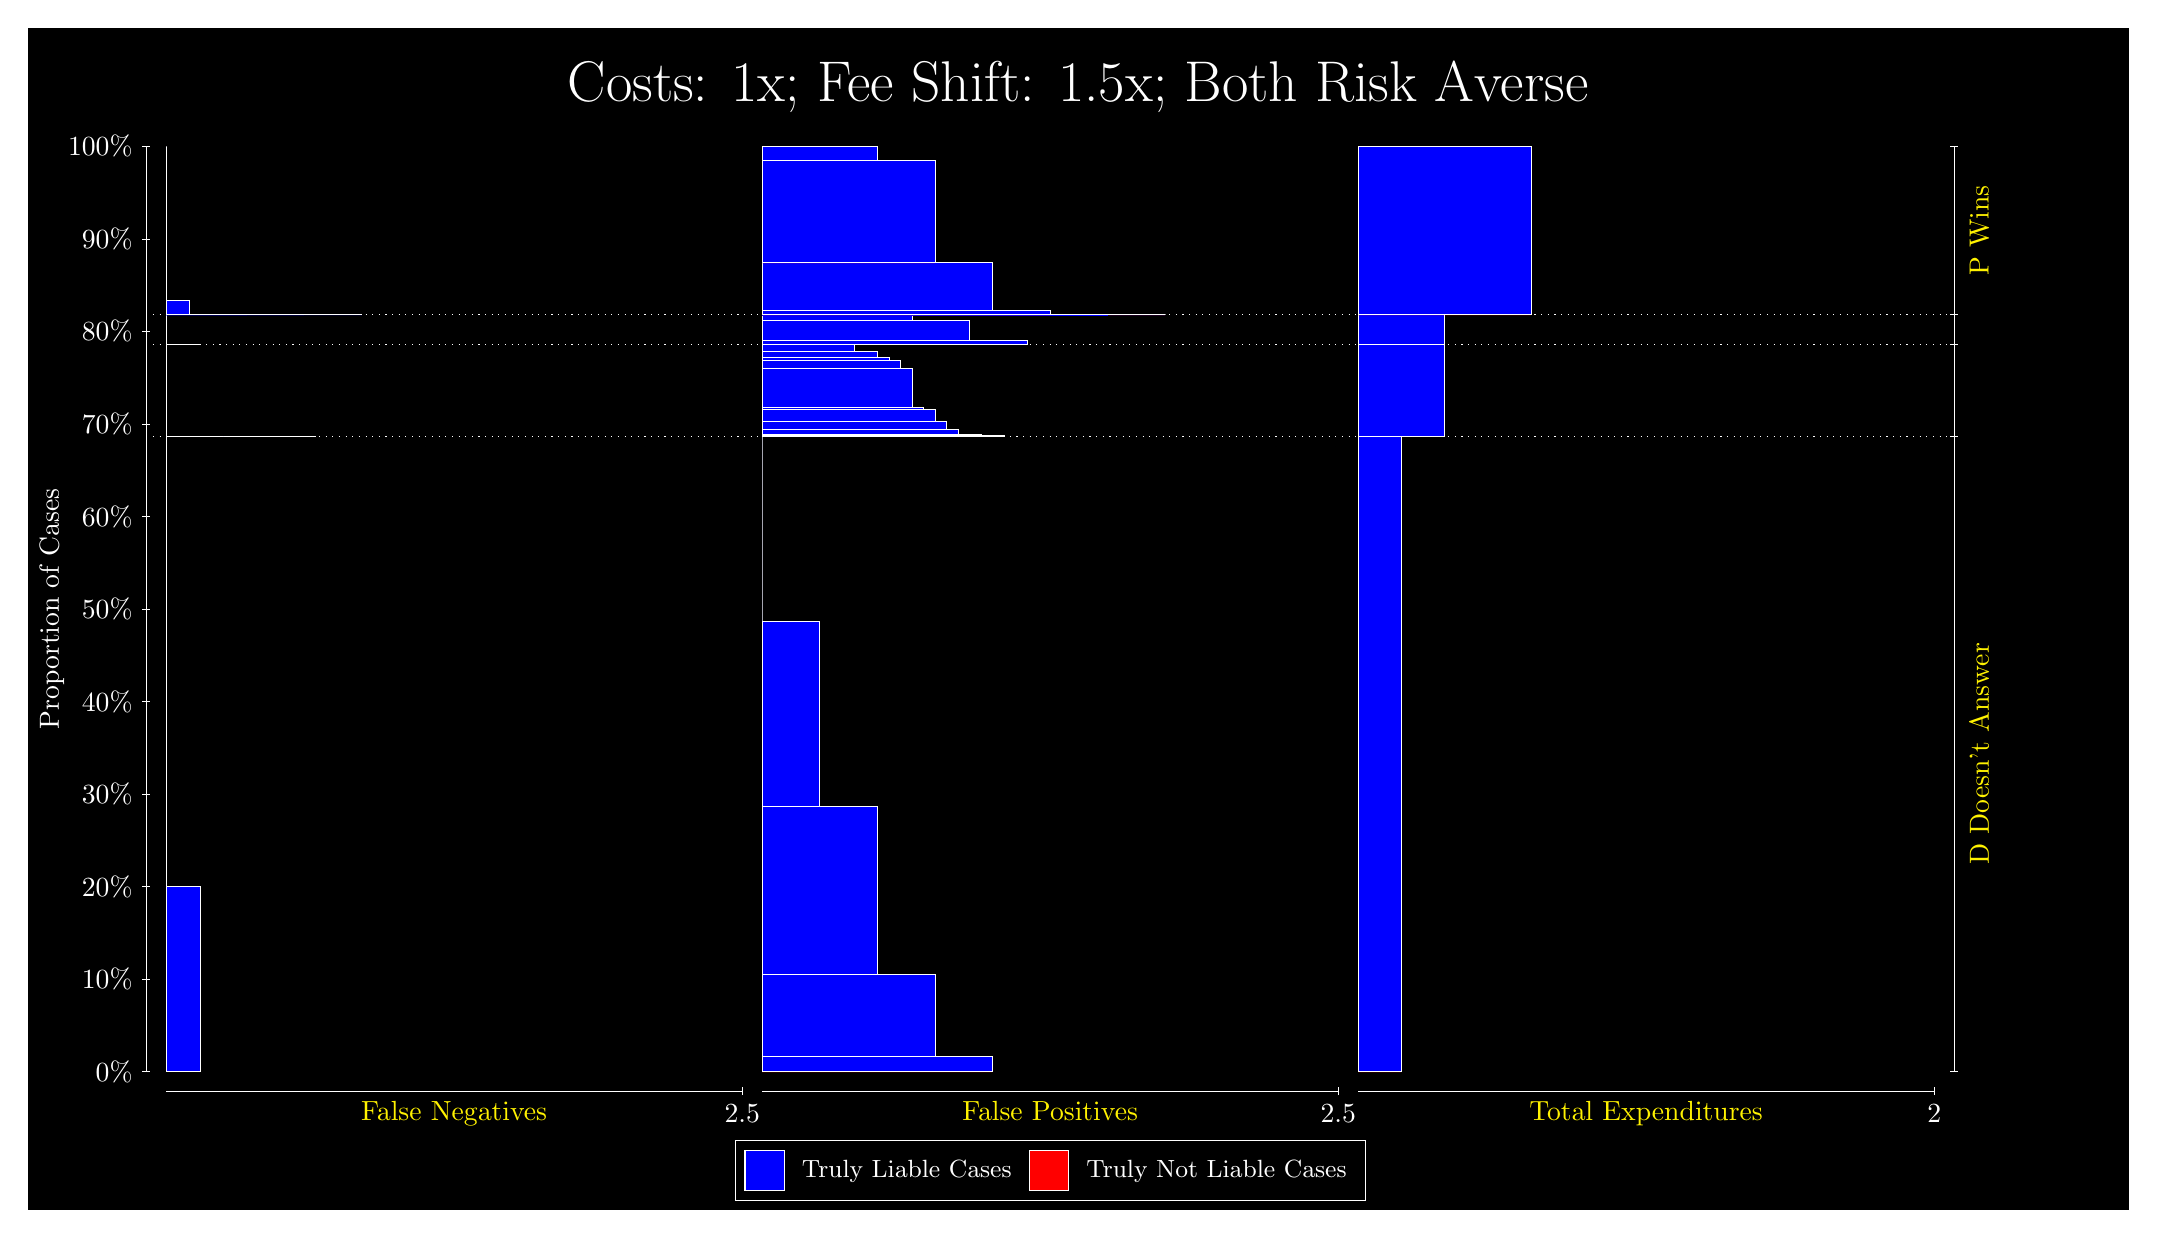
\begin{tikzpicture}
\draw[fill=black] (0,0) rectangle (26.667,15);
\draw[text=white] (0,13.5) rectangle (26.667,15) node[midway] {\huge Costs: 1x; Fee Shift: 1.5x; Both Risk Averse};
\draw[white, very thin] (1.5,1.75) -- (1.5,13.5);
\node[rotate=90, text=white, anchor=center] at (0.3, 7.625) {Proportion of Cases};
\draw[white, very thin] (1.45,1.75) -- (1.55,1.75);
\node[text=white, anchor=east] at (1.45, 1.75) {0\%};
\draw[white, very thin] (1.45,2.925) -- (1.55,2.925);
\node[text=white, anchor=east] at (1.45, 2.925) {10\%};
\draw[white, very thin] (1.45,4.1) -- (1.55,4.1);
\node[text=white, anchor=east] at (1.45, 4.1) {20\%};
\draw[white, very thin] (1.45,5.275) -- (1.55,5.275);
\node[text=white, anchor=east] at (1.45, 5.275) {30\%};
\draw[white, very thin] (1.45,6.45) -- (1.55,6.45);
\node[text=white, anchor=east] at (1.45, 6.45) {40\%};
\draw[white, very thin] (1.45,7.625) -- (1.55,7.625);
\node[text=white, anchor=east] at (1.45, 7.625) {50\%};
\draw[white, very thin] (1.45,8.8) -- (1.55,8.8);
\node[text=white, anchor=east] at (1.45, 8.8) {60\%};
\draw[white, very thin] (1.45,9.975) -- (1.55,9.975);
\node[text=white, anchor=east] at (1.45, 9.975) {70\%};
\draw[white, very thin] (1.45,11.15) -- (1.55,11.15);
\node[text=white, anchor=east] at (1.45, 11.15) {80\%};
\draw[white, very thin] (1.45,12.325) -- (1.55,12.325);
\node[text=white, anchor=east] at (1.45, 12.325) {90\%};
\draw[white, very thin] (1.45,13.5) -- (1.55,13.5);
\node[text=white, anchor=east] at (1.45, 13.5) {100\%};

\draw[white, very thin] (24.457,1.75) -- (24.457,13.5);
\draw[white, very thin] (24.407,1.75) -- (24.507,1.75);
\node[anchor=west] at (24.407, 1.75) {};
\draw[white, very thin] (24.407,9.8185) -- (24.507,9.8185);
\node[anchor=west] at (24.407, 9.8185) {};
\draw[white, very thin] (24.407,10.987) -- (24.507,10.987);
\node[anchor=west] at (24.407, 10.987) {};
\draw[white, very thin] (24.407,11.363) -- (24.507,11.363);
\node[anchor=west] at (24.407, 11.363) {};
\draw[white, very thin] (24.407,13.5) -- (24.507,13.5);
\node[anchor=west] at (24.407, 13.5) {};

\draw[white, very thin, fill=blue] (1.75,1.75) rectangle (2.1891,4.0999);
\draw[white, very thin, fill=red] (1.75,4.0999) rectangle (1.75,4.0999);
\draw[white, very thin, fill=blue] (1.75,4.0999) rectangle (1.75,9.8185);
\draw[white, very thin, fill=blue] (1.75,9.8185) rectangle (3.6529,9.8185);
\draw[white, very thin, fill=blue] (1.75,9.8185) rectangle (3.3602,9.8185);
\draw[white, very thin, fill=blue] (1.75,9.8185) rectangle (3.0674,9.8185);
\draw[white, very thin, fill=blue] (1.75,9.8185) rectangle (2.921,9.8185);
\draw[white, very thin, fill=blue] (1.75,9.8185) rectangle (2.7746,9.8185);
\draw[white, very thin, fill=blue] (1.75,9.8185) rectangle (2.6283,9.8185);
\draw[white, very thin, fill=blue] (1.75,9.8185) rectangle (2.4819,9.8185);
\draw[white, very thin, fill=blue] (1.75,9.8185) rectangle (2.3355,9.8185);
\draw[white, very thin, fill=blue] (1.75,9.8185) rectangle (2.1891,9.82);
\draw[white, very thin, fill=blue] (1.75,9.82) rectangle (2.0428,9.82);
\draw[white, very thin, fill=blue] (1.75,9.82) rectangle (1.8964,9.822);
\draw[white, very thin, fill=red] (1.75,9.822) rectangle (1.75,9.822);
\draw[white, very thin, fill=blue] (1.75,9.822) rectangle (1.75,10.987);
\draw[white, very thin, fill=blue] (1.75,10.987) rectangle (2.1891,10.987);
\draw[white, very thin, fill=red] (1.75,10.987) rectangle (1.75,10.987);
\draw[white, very thin, fill=blue] (1.75,10.987) rectangle (1.75,11.363);
\draw[white, very thin, fill=blue] (1.75,11.363) rectangle (4.2384,11.363);
\draw[white, very thin, fill=blue] (1.75,11.363) rectangle (3.5065,11.363);
\draw[white, very thin, fill=blue] (1.75,11.363) rectangle (2.7746,11.363);
\draw[white, very thin, fill=blue] (1.75,11.363) rectangle (2.7746,11.365);
\draw[white, very thin, fill=blue] (1.75,11.365) rectangle (2.0428,11.365);
\draw[white, very thin, fill=blue] (1.75,11.365) rectangle (2.0428,11.544);
\draw[white, very thin, fill=red] (1.75,11.544) rectangle (1.75,11.544);
\draw[white, very thin, fill=blue] (1.75,11.544) rectangle (1.75,13.5);
\draw[white, very thin, fill=red] (9.3189,1.75) rectangle (12.246,1.75);
\draw[white, very thin, fill=blue] (9.3189,1.75) rectangle (12.246,1.9386);
\draw[white, very thin, fill=blue] (9.3189,1.9386) rectangle (11.515,2.9877);
\draw[white, very thin, fill=blue] (9.3189,2.9877) rectangle (10.783,5.1204);
\draw[white, very thin, fill=blue] (9.3189,5.1204) rectangle (10.051,7.4686);
\draw[white, very thin, fill=blue] (9.3189,7.4686) rectangle (9.3189,9.8185);
\draw[white, very thin, fill=red] (9.3189,9.8185) rectangle (12.393,9.8185);
\draw[white, very thin, fill=blue] (9.3189,9.8185) rectangle (12.393,9.8348);
\draw[white, very thin, fill=red] (9.3189,9.8348) rectangle (12.1,9.8348);
\draw[white, very thin, fill=blue] (9.3189,9.8348) rectangle (12.1,9.8413);
\draw[white, very thin, fill=red] (9.3189,9.8413) rectangle (11.807,9.8413);
\draw[white, very thin, fill=blue] (9.3189,9.8413) rectangle (11.807,9.9089);
\draw[white, very thin, fill=blue] (9.3189,9.9089) rectangle (11.661,10.008);
\draw[white, very thin, fill=red] (9.3189,10.008) rectangle (11.515,10.008);
\draw[white, very thin, fill=blue] (9.3189,10.008) rectangle (11.515,10.156);
\draw[white, very thin, fill=blue] (9.3189,10.156) rectangle (11.368,10.184);
\draw[white, very thin, fill=red] (9.3189,10.184) rectangle (11.222,10.184);
\draw[white, very thin, fill=blue] (9.3189,10.184) rectangle (11.222,10.684);
\draw[white, very thin, fill=blue] (9.3189,10.684) rectangle (11.075,10.785);
\draw[white, very thin, fill=blue] (9.3189,10.785) rectangle (10.929,10.819);
\draw[white, very thin, fill=blue] (9.3189,10.819) rectangle (10.783,10.894);
\draw[white, very thin, fill=blue] (9.3189,10.894) rectangle (10.636,10.895);
\draw[white, very thin, fill=blue] (9.3189,10.895) rectangle (10.49,10.98);
\draw[white, very thin, fill=blue] (9.3189,10.98) rectangle (10.344,10.984);
\draw[white, very thin, fill=blue] (9.3189,10.984) rectangle (10.197,10.984);
\draw[white, very thin, fill=blue] (9.3189,10.984) rectangle (10.051,10.986);
\draw[white, very thin, fill=blue] (9.3189,10.986) rectangle (9.9044,10.986);
\draw[white, very thin, fill=blue] (9.3189,10.986) rectangle (9.758,10.987);
\draw[white, very thin, fill=blue] (9.3189,10.987) rectangle (9.6116,10.987);
\draw[white, very thin, fill=blue] (9.3189,10.987) rectangle (9.4652,10.987);
\draw[white, very thin, fill=blue] (9.3189,10.987) rectangle (9.3189,10.987);
\draw[white, very thin, fill=red] (9.3189,10.987) rectangle (12.686,10.987);
\draw[white, very thin, fill=blue] (9.3189,10.987) rectangle (12.686,11.039);
\draw[white, very thin, fill=blue] (9.3189,11.039) rectangle (11.954,11.29);
\draw[white, very thin, fill=blue] (9.3189,11.29) rectangle (11.222,11.362);
\draw[white, very thin, fill=blue] (9.3189,11.362) rectangle (10.49,11.363);
\draw[white, very thin, fill=blue] (9.3189,11.363) rectangle (9.758,11.363);
\draw[white, very thin, fill=red] (9.3189,11.363) rectangle (14.442,11.363);
\draw[white, very thin, fill=blue] (9.3189,11.363) rectangle (14.442,11.363);
\draw[white, very thin, fill=red] (9.3189,11.363) rectangle (13.71,11.363);
\draw[white, very thin, fill=blue] (9.3189,11.363) rectangle (13.71,11.364);
\draw[white, very thin, fill=red] (9.3189,11.364) rectangle (12.978,11.364);
\draw[white, very thin, fill=blue] (9.3189,11.364) rectangle (12.978,11.422);
\draw[white, very thin, fill=red] (9.3189,11.422) rectangle (12.246,11.422);
\draw[white, very thin, fill=blue] (9.3189,11.422) rectangle (12.246,12.023);
\draw[white, very thin, fill=red] (9.3189,12.023) rectangle (11.515,12.023);
\draw[white, very thin, fill=blue] (9.3189,12.023) rectangle (11.515,13.319);
\draw[white, very thin, fill=blue] (9.3189,13.319) rectangle (10.783,13.498);
\draw[white, very thin, fill=blue] (9.3189,13.498) rectangle (10.051,13.5);
\draw[white, very thin, fill=blue] (9.3189,13.5) rectangle (9.3189,13.5);
\draw[white, very thin, fill=red] (16.888,1.75) rectangle (17.437,1.75);
\draw[white, very thin, fill=blue] (16.888,1.75) rectangle (17.437,9.8185);
\draw[white, very thin, fill=red] (16.888,9.8185) rectangle (17.986,9.8185);
\draw[white, very thin, fill=blue] (16.888,9.8185) rectangle (17.986,10.987);
\draw[white, very thin, fill=red] (16.888,10.987) rectangle (17.986,10.987);
\draw[white, very thin, fill=blue] (16.888,10.987) rectangle (17.986,11.363);
\draw[white, very thin, fill=red] (16.888,11.363) rectangle (19.083,11.363);
\draw[white, very thin, fill=blue] (16.888,11.363) rectangle (19.083,13.5);
\draw[white, dotted] (1.5,9.8185) -- (24.457,9.8185);
\draw[white, dotted] (1.5,10.987) -- (24.457,10.987);
\draw[white, dotted] (1.5,11.363) -- (24.457,11.363);
\draw[white, very thin] (1.75,1.5) -- (9.0689,1.5);
\node[text=yellow, anchor=north] at (5.4094, 1.5) {False Negatives};
\draw[white, very thin] (9.0689,1.45) -- (9.0689,1.55);
\node[text=white, anchor=north] at (9.0689, 1.45) {2.5};

\draw[white, very thin] (9.3189,1.5) -- (16.638,1.5);
\node[text=yellow, anchor=north] at (12.978, 1.5) {False Positives};
\draw[white, very thin] (16.638,1.45) -- (16.638,1.55);
\node[text=white, anchor=north] at (16.638, 1.45) {2.5};

\draw[white, very thin] (16.888,1.5) -- (24.207,1.5);
\node[text=yellow, anchor=north] at (20.547, 1.5) {Total Expenditures};
\draw[white, very thin] (24.207,1.45) -- (24.207,1.55);
\node[text=white, anchor=north] at (24.207, 1.45) {2};

\node[text=yellow, centered, rotate=90] at (24.777, 5.7842) {D Doesn't Answer};


\node[text=yellow, centered, rotate=90] at (24.777, 12.431) {P Wins};

\draw (12.978300999999998,1.5) node[draw=none] (baseCoordinate) {};
\begin{scope}[align=center]
        \matrix[scale=0.5, draw=white, below=0.5cm of baseCoordinate, nodes={draw}, column sep=0.1cm]{
            \node[rectangle, draw, minimum width=0.5cm, minimum height=0.5cm, fill=blue] {}; &
            \node[draw=none, font=\small, text=white] (B) {Truly Liable Cases}; &
            \node[rectangle, draw, minimum width=0.5cm, minimum height=0.5cm, fill=red] {}; &
            \node[draw=none, font=\small, text=white] (B) {Truly Not Liable Cases}; \\
            };
\end{scope}

\end{tikzpicture}
\end{document}